%%
%% Preamble
%%
% \documentclass{<something>} must begin each LaTeX document
\documentclass[11pt,twoside]{MPIthesis}
% Packages are extensions to the basic LaTeX functions. Whatever you
% want to typeset, there is probably a package out there for it.
% Chemistry (chemtex), screenplays, you name it.
% Check out CTAN to see: http://www.ctan.org/
%%
\usepackage{graphicx,latexsym}
\usepackage{amsmath}
\usepackage{amssymb,amsthm}
\usepackage{longtable,booktabs,setspace}
\usepackage{chemarr} %% Useful for one reaction arrow, useless if you're not a chem major
\usepackage[hyphens]{url}
% Added by CII
\usepackage{hyperref}
\usepackage{lmodern}
\usepackage{float}
\floatplacement{figure}{H}
% End of CII addition
\usepackage{rotating}
%% VB ADD
\usepackage{pdfpages} % to be able to include pdf files as appendices (\includepdf[pages={-}]{myfile.pdf})
%% // VB ADD

% Next line commented out by CII
%%% \usepackage{natbib}
% Comment out the natbib line above and uncomment the following two lines to use the new
% biblatex-chicago style, for Chicago A. Also make some changes at the end where the
% bibliography is included.
%\usepackage{biblatex-chicago}
%\bibliography{thesis}


% Added by CII (Thanks, Hadley!)
% Use ref for internal links
\renewcommand{\hyperref}[2][???]{\autoref{#1}}
\def\chapterautorefname{Chapter}
\def\sectionautorefname{Section}
\def\subsectionautorefname{Subsection}
% End of CII addition

% Added by CII
\usepackage{caption}
\captionsetup{width=5in}
% End of CII addition

% \usepackage{times} % other fonts are available like times, bookman, charter, palatino

% Syntax highlighting #22

% To pass between YAML and LaTeX the dollar signs are added by CII
\title{Computational epigenomics study of the Male-Specific Lethal complex in
flies and mammals}
\author{Vivek BHARDWAJ}
\date{20 September, 2018}
\advisor{Dr.~Asifa AKHTAR}
\institution{Max Planck Institute of Immunobiology and Epigenetics}
\secondreviewer{Dr.~Thomas Manke}
\thirdreviewer{Dr.~Giorgos Pyrowolakis}
\decan{Mr.~Decan}
\promotionsvorsitzender{Dr.~Someone}


%%% Remember to use the correct department!
\department{}

% Added by CII
%%% Copied from knitr
%% maxwidth is the original width if it's less than linewidth
%% otherwise use linewidth (to make sure the graphics do not exceed the margin)
\makeatletter
\def\maxwidth{ %
  \ifdim\Gin@nat@width>\linewidth
    \linewidth
  \else
    \Gin@nat@width
  \fi
}
\makeatother

\renewcommand{\contentsname}{Contents}%VB
% End of CII addition

\setlength{\parskip}{0pt}

% Added by CII
  %\setlength{\parskip}{\baselineskip}
  \usepackage[parfill]{parskip}

\providecommand{\tightlist}{%
  \setlength{\itemsep}{0pt}\setlength{\parskip}{0pt}}

\Acknowledgements{
This thesis would not be complete without the help and support of people
from both the Akhtar Lab and Manke group at the MPI-IE. I am grateful to
both my supervisors Dr.~Asifa Akhtar and Dr.~Thomas Manke for trusting
my abilities and allowing me to work with them. Asifa provided me with
all the independence I desired to work on my projects and to collaborate
with the people in the lab. Discussions with her provided me the
motivation and ability to see the significance of the work I was doing.
Thomas has always been available for me to discuss all sorts of issues
and provided me with the support and encouragement I needed to improve
my skills and prepare for the next steps in my career. Opting for this
co-supervision was the best choice I could have made for my PhD.

All of my works presented here have been done in collaboration, and
would not be completed without the efforts and insights of those
involved. I would like to thank :

Fidel, who taught me HiC analysis and mentored me during our
collaboration on the HiC project. Due to HiCExplorer and deepTools
projects, I was pushed out of my comfort zone to learn Python and to
adopt reproducible workflows for my analysis. I glady cherish all the
discussions with Fidel during work as well as during our Sunday morning
run. Giuseppe, for initiating the wonderful collaborations on the
Drosophila projects, and for all the helpful discussions over the years.
Raed, for working with me on the mammalian MSL2 project. Ibrahim and
Tugce for initiating the collaboration on the mammalian MLE project, and
finally Bilal and Ken for other independent projects. I would like to
thank all the people at the Bioinformatics Unit for providing me with
such a wonderful and interactive working environment, useful
discussions, and fun collaborations. The deep-sequencing unit for
producing the great quality data, and people in the Akhtar lab for all
the discussions as well as fun activities outside work. Finally I want
to thank my TAC members Ritwick Sawarkar and Michael Stadler for the
support and discussions during my TAC.
}

% End of CII addition
%%
%% End Preamble
%%
%
\begin{document}

%% VB add
  \maketitle

\makepagetwo
%% \VB add

% Everything below added by CII
\frontmatter % this stuff will be roman-numbered
\pagestyle{empty} % this removes page numbers from the frontmatter
  \begin{acknowledgements}
    This thesis would not be complete without the help and support of people
    from both the Akhtar Lab and Manke group at the MPI-IE. I am grateful to
    both my supervisors Dr.~Asifa Akhtar and Dr.~Thomas Manke for trusting
    my abilities and allowing me to work with them. Asifa provided me with
    all the independence I desired to work on my projects and to collaborate
    with the people in the lab. Discussions with her provided me the
    motivation and ability to see the significance of the work I was doing.
    Thomas has always been available for me to discuss all sorts of issues
    and provided me with the support and encouragement I needed to improve
    my skills and prepare for the next steps in my career. Opting for this
    co-supervision was the best choice I could have made for my PhD.
    
    All of my works presented here have been done in collaboration, and
    would not be completed without the efforts and insights of those
    involved. I would like to thank :
    
    Fidel, who taught me HiC analysis and mentored me during our
    collaboration on the HiC project. Due to HiCExplorer and deepTools
    projects, I was pushed out of my comfort zone to learn Python and to
    adopt reproducible workflows for my analysis. I glady cherish all the
    discussions with Fidel during work as well as during our Sunday morning
    run. Giuseppe, for initiating the wonderful collaborations on the
    Drosophila projects, and for all the helpful discussions over the years.
    Raed, for working with me on the mammalian MSL2 project. Ibrahim and
    Tugce for initiating the collaboration on the mammalian MLE project, and
    finally Bilal and Ken for other independent projects. I would like to
    thank all the people at the Bioinformatics Unit for providing me with
    such a wonderful and interactive working environment, useful
    discussions, and fun collaborations. The deep-sequencing unit for
    producing the great quality data, and people in the Akhtar lab for all
    the discussions as well as fun activities outside work. Finally I want
    to thank my TAC members Ritwick Sawarkar and Michael Stadler for the
    support and discussions during my TAC.
  \end{acknowledgements}
  \hypersetup{linkcolor=black}
  \setcounter{tocdepth}{2}
  \tableofcontents


  \listoffigures
  \begin{abstract}
    In various species, sex determination is associated with an imbalance in
    the number of sex chromosomes between males and females. In Drosophila,
    this imbalance is corrected by an chromosome-level epigenetic phenomenon
    resulting in the upregulation of gene expression on the single male X
    chromosome. This phenomenon, referred to as dosage compensation,
    requires the Male-specific lethal (MSL) complex. The 3D conformation of
    the X-chromosome guides the spreading of the MSL complex, depositing
    histone (H4K16) acetylation on genes. On the other hand, mammalian
    dosage compensation occurs via X inactivation in females, and the role
    of MSL complex in mammals is poorly understood.
    
    The aim of my project was to provide insights into the functions of the
    MSL complex in flies and mammals through computational epigenomics
    approach. This involved development of methods and tools for analysis of
    chromosome conformation and promoter-profiling data, and their
    integration with other transcriptomic and epigenetic data. Softwares
    such as HiCExplorer, icetea and deepTools2 were developed to facilitate
    this, and workflows for reproducible analysis were implemented as part
    of the snakePipes package. Application of our methods on HiC data in
    flies revealed that chromatin domains influence gene transcription, and
    validated previous observation on clustering of MSL2 sites in 3D space.
    Analysis of the MSL complex member MLE through promoter profiling
    identified a catalogue of MLE sensitive and insensitive promoters at the
    male X-chromosome and the difference in MLE action between sexes.
    Analysis of mammalian ortholog of MLE revealed it's novel function in
    regulation of Alu transposons independent of the MSL complex, while the
    analysis of other members of the mammalian MSL complex showed that MSLs
    are involved in transcriptional regulation of genes on X chromosome in
    an allele-specific manner.
    
    In summary, we gained new insights into the functions of the MSL complex
    through analysis and integration of multiple epigenomic and
    transcriptomic data. This study would motivate further studies utilizing
    integrative epigenomics to understand the functions of MSLs as well as
    other regulators of transcription.
  \end{abstract}
\mainmatter % here the regular arabic numbering starts
\pagestyle{fancyplain} % turns page numbering back on

\chapter*{Abbreviations}\label{abbreviations}
\addcontentsline{toc}{chapter}{Abbreviations}
\begin{tabular}{ll}
\toprule
Term & Abbreviation\\
\midrule
Long-term memory & LTM\\
Short-term memory & STM\\
Working memory & WM\\
\bottomrule
\end{tabular}
\chapter{Introduction}\label{introduction}

\chapter{Results and discussion}\label{results-and-discussion}

\appendix

\chapter{Publications and
Manuscripts}\label{publications-and-manuscripts}

\section{Analysis of chromosome conformation in
flies}\label{analysis-of-chromosome-conformation-in-flies}

I contributed to the development of HiCExplorer and HiCBrowser (led by
Fidel Ramirez), and developed the Chorogenome Navigator resource. I
performed the analysis of motif combinations and boundary strength,
prediction of motifs, and relationship of TAD boundary and transcription
(Fig 2, S2, 4, S4, 5 and S5). Together with Fidel Ramirez and Thomas
Manke I devised, wrote, and revised the manuscript.

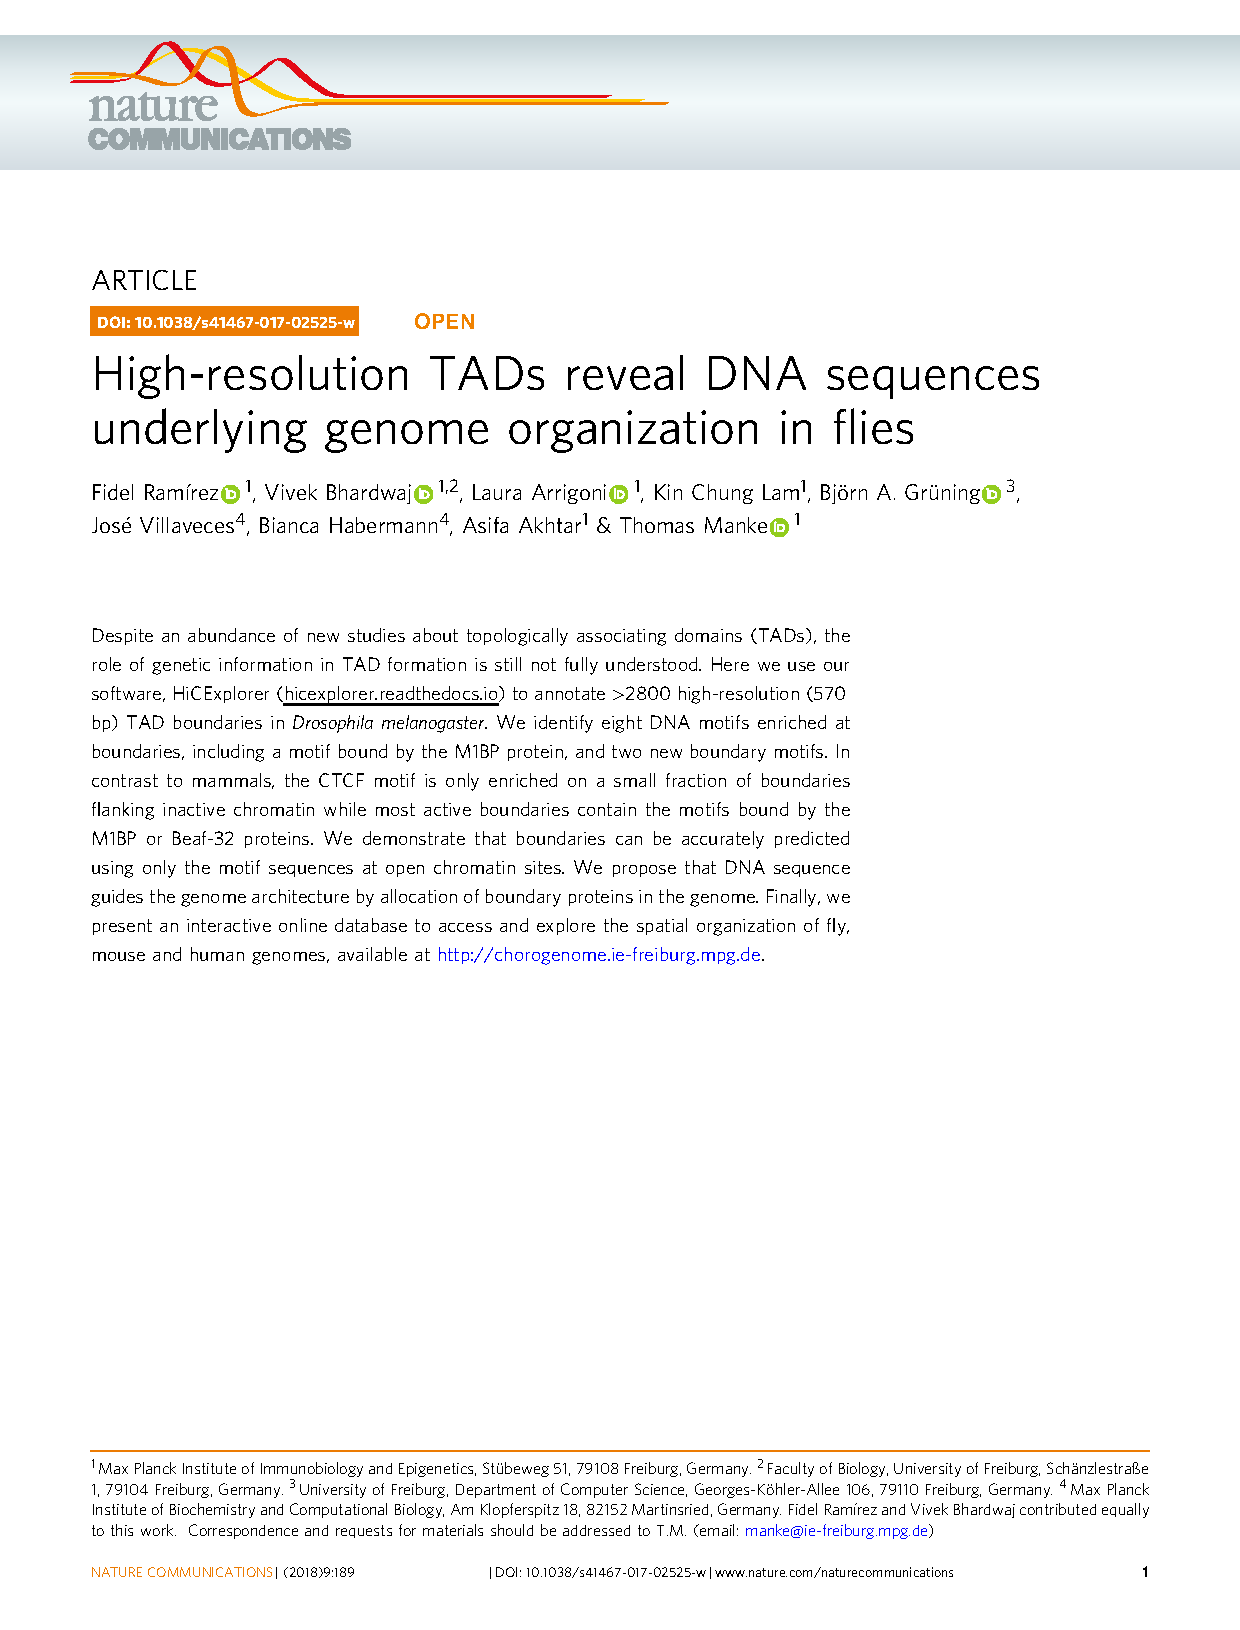
\includepdf[scale=0.9,pages=-,pagecommand={}, offset=0.3cm 0cm]{manuscripts/NatComm_2018_article.pdf}

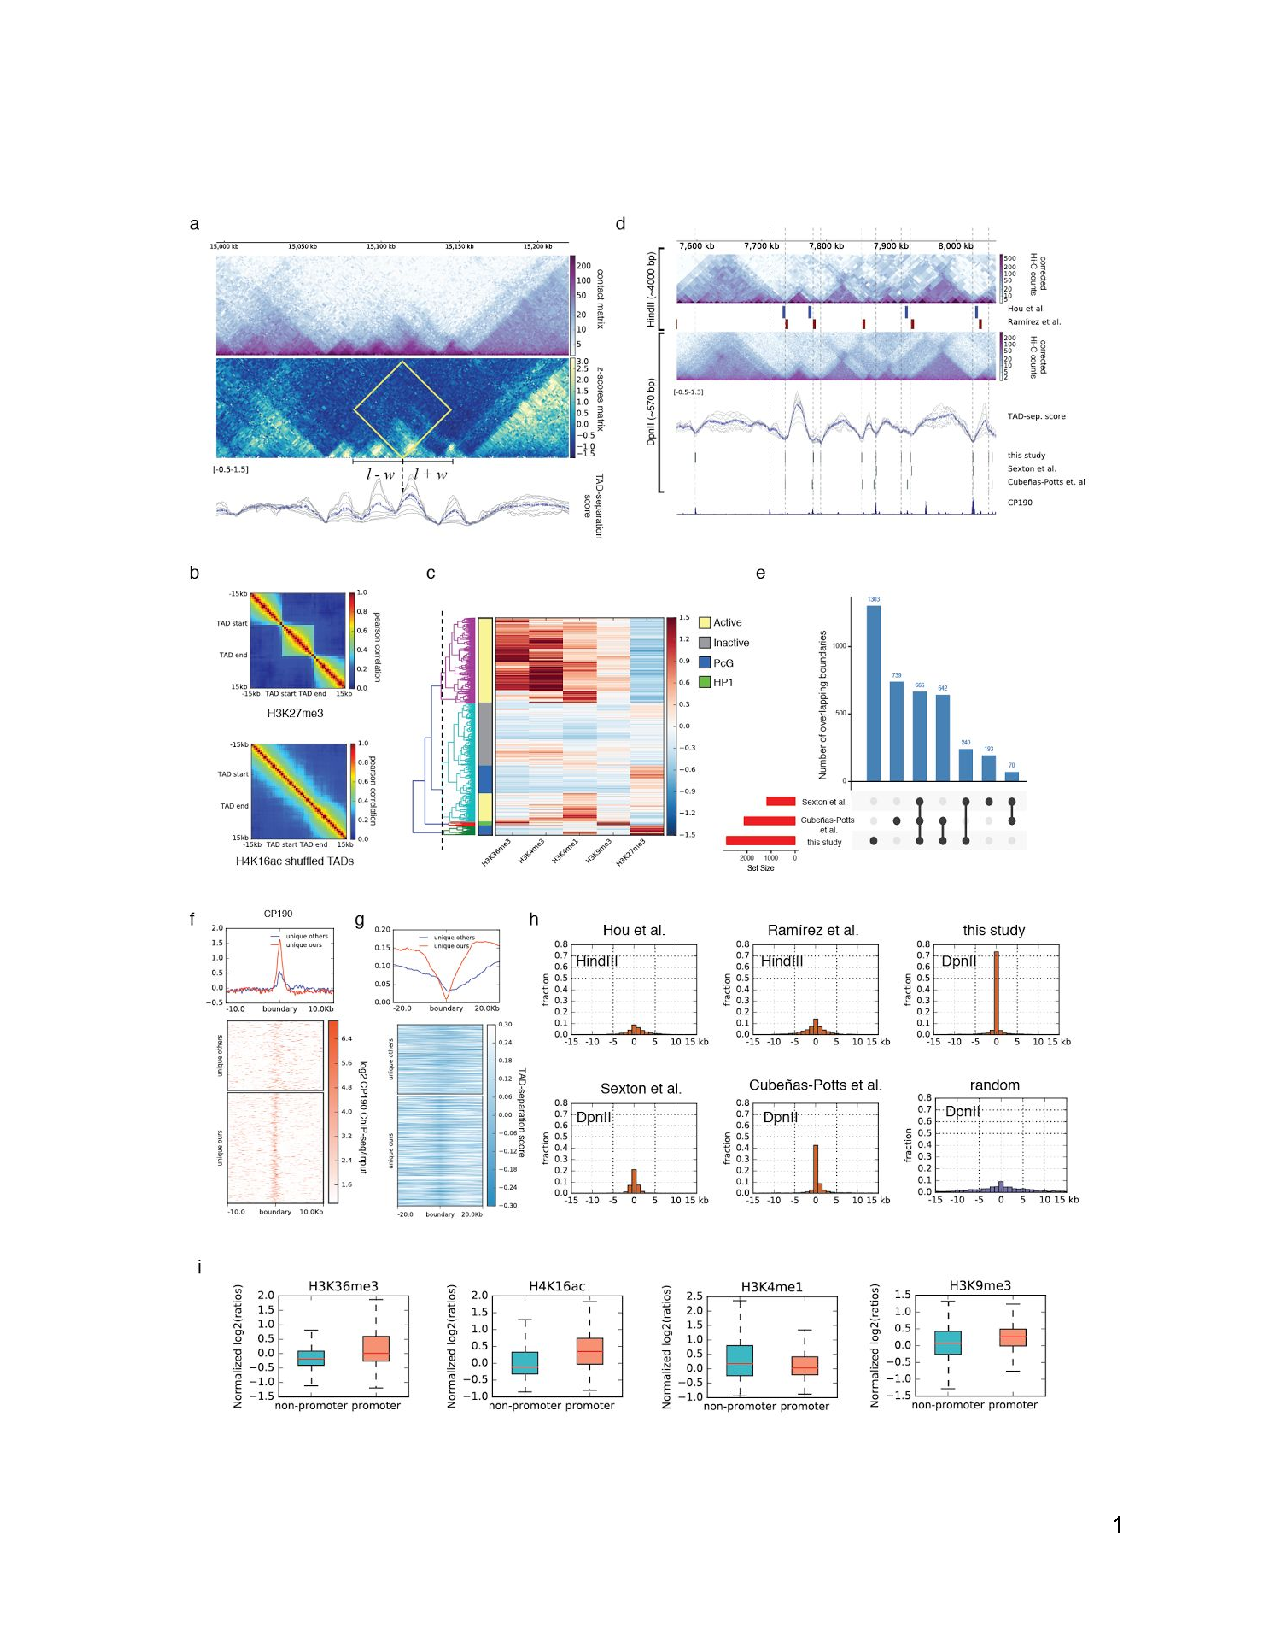
\includepdf[scale=0.9,pages=-,pagecommand={}, offset=0.3cm 0cm]{manuscripts/NatComm_2018_supple.pdf}

\section{Galaxy HiCExplorer}\label{galaxy-hicexplorer}

I contributed to the development of HiCExplorer and designed the
template workflow for the galaxy web server. I contributed to the
writing and revision of the manuscript along with Joachim Wolff and
other authors.

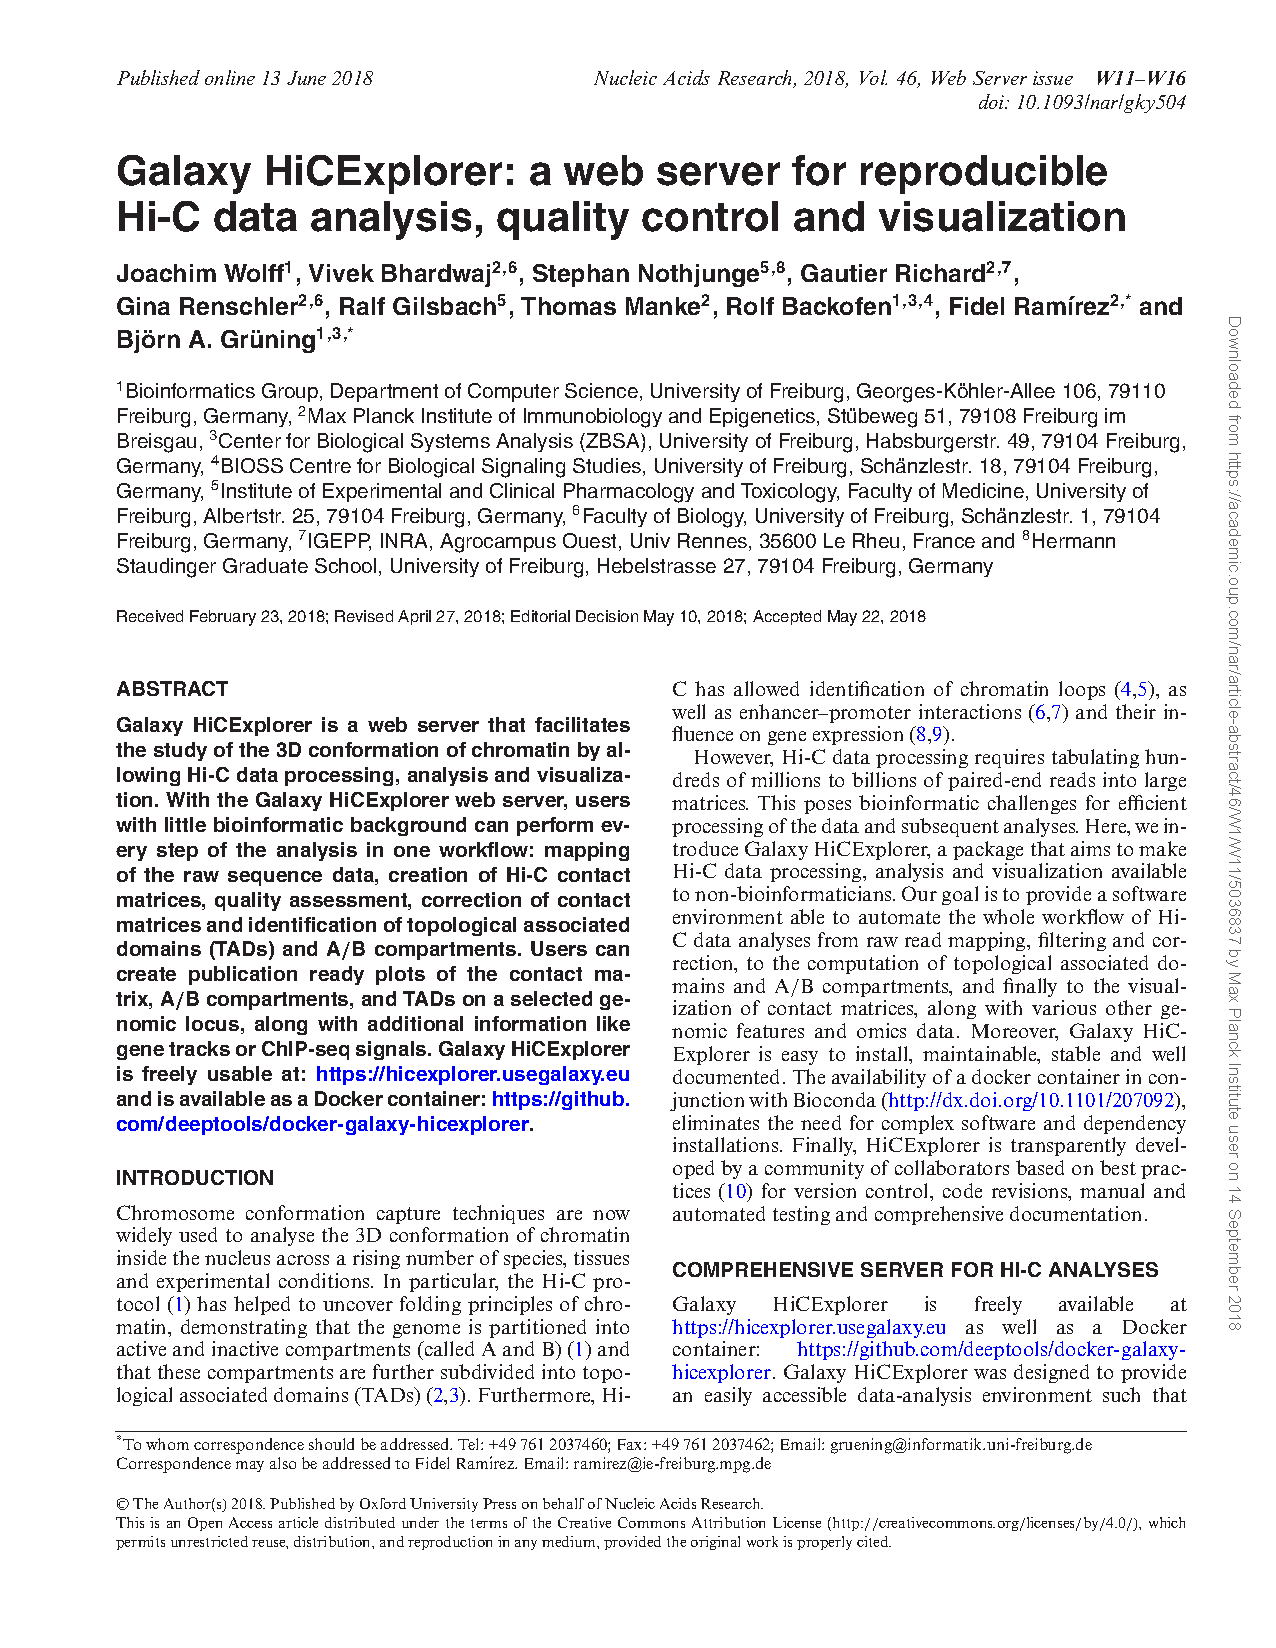
\includepdf[scale=0.9,pages=-,pagecommand={}, offset=0.3cm 0cm]{manuscripts/NAR_2018_article.pdf}

\section{Analysis of dosage compensation in flies via
promoter-profiling}\label{analysis-of-dosage-compensation-in-flies-via-promoter-profiling}

I contributed to the development of the MAPCap protocol by providing the
analysis input, where all the experiments were performed by Giuseppe
Semplicio. I developed the icetea bioconductor package and performed all
the analysis presented in the paper, made the figures and wrote the
manuscript with input from Giuseppe Semplicio.

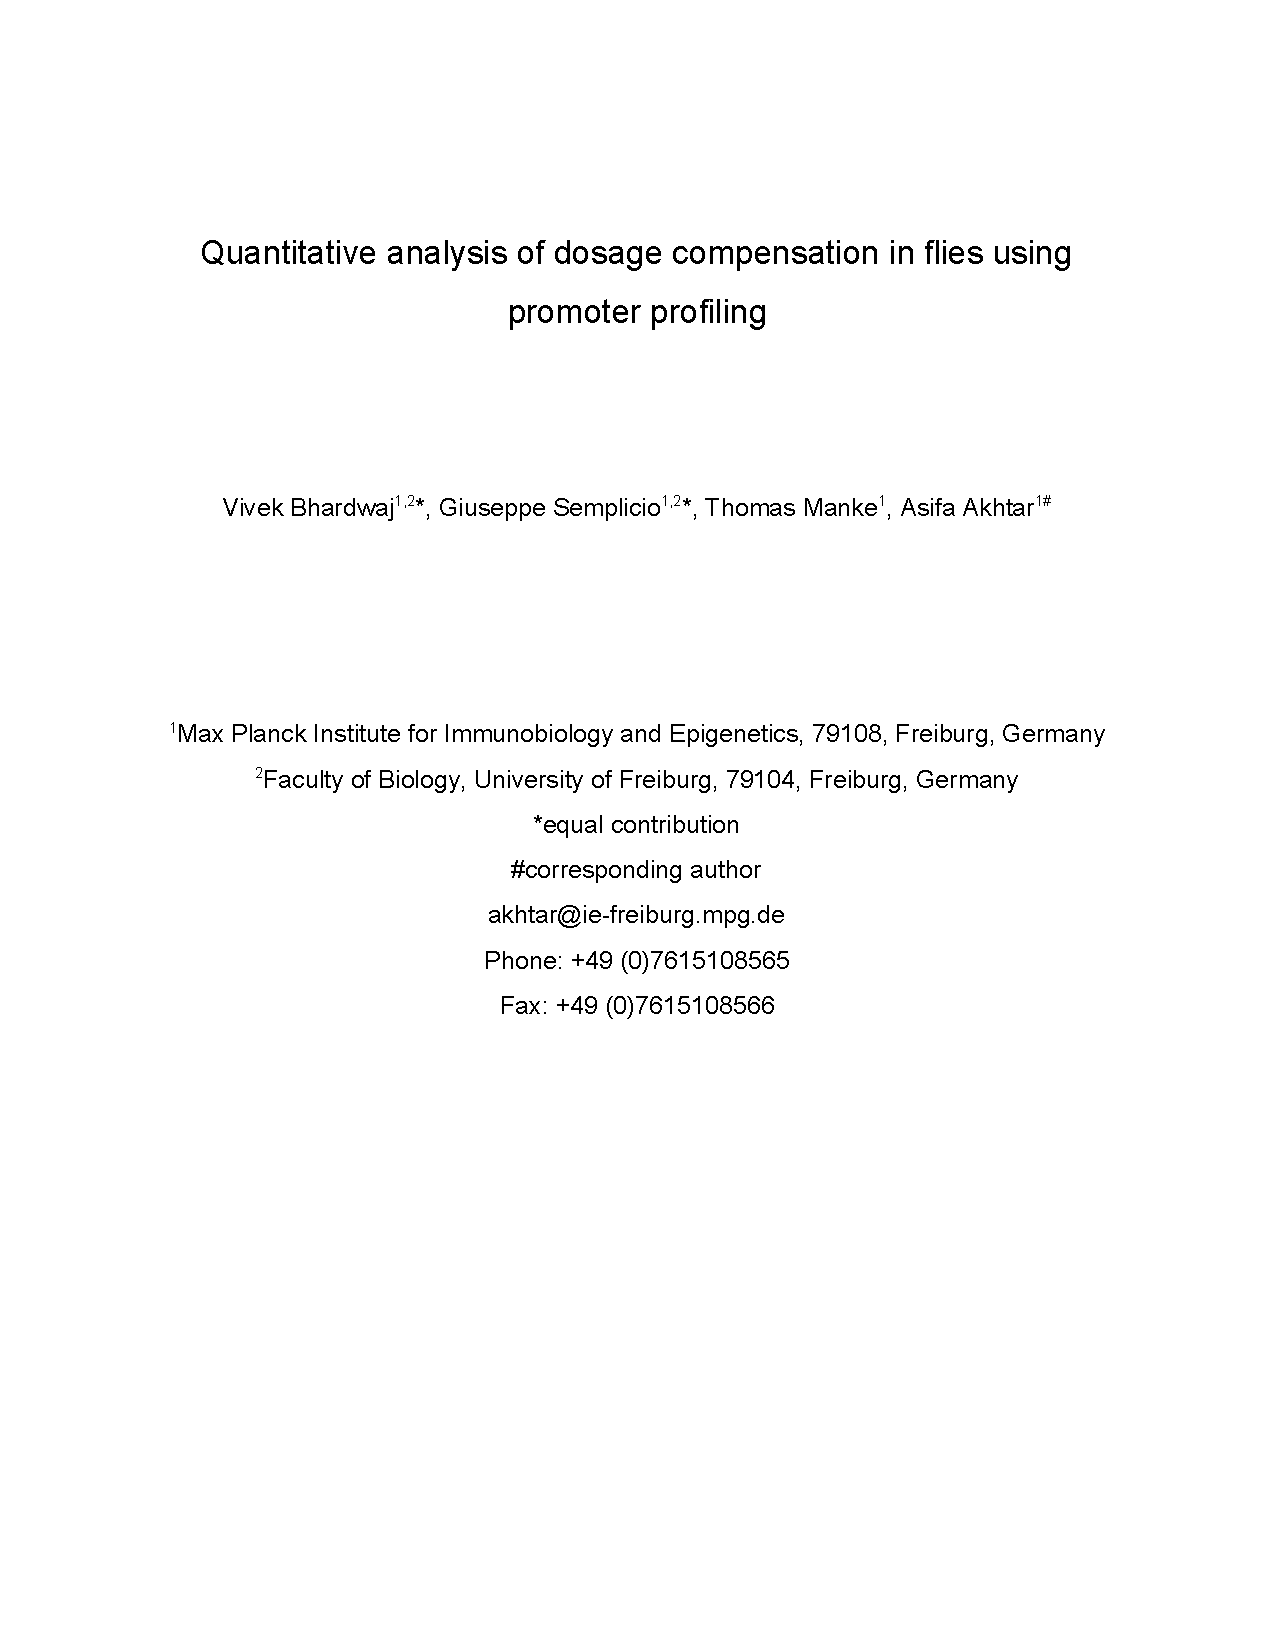
\includepdf[scale=0.9,pages=-,pagecommand={}, offset=0.3cm 0cm]{manuscripts/mapcap_paper_14-09-2018.pdf}

\section{Interaction of MLE ortholog DHX9 with Alu elements in the human
genome}\label{interaction-of-mle-ortholog-dhx9-with-alu-elements-in-the-human-genome}

I performed the analysis of UV-CLAP data for estimation of Alu
enrichment (Extended data Fig. 2 and 3) and performed the RNA-seq
analysis for detection of differential expression, splicing, circular
RNAs and RNA editing (Fig. 2a, 2b, 3a, Extended Data Figure 6, 7, 10). I
contributed to the writing and revision of the manuscript along with
Tugce Aktas, Ibrahim Ilik, Asifa Akhtar and other authors.

\includepdf[scale=0.9,pages=-,pagecommand={}, offset=0.3cm 0cm]{manuscripts/Nature_2017_article_supple.pdf}

\section{Update of the deepTools toolkit for exploring deep-sequencing
data}\label{update-of-the-deeptools-toolkit-for-exploring-deep-sequencing-data}

I contributed to the development of deepTools2 (led by Fidel Ramirez and
Devon Ryan) through features and bugfixes, and to the testing and update
of the documentation and the galaxy server. I helped with the writing
and revision of the manuscript by Fidel Ramirez and other authors.

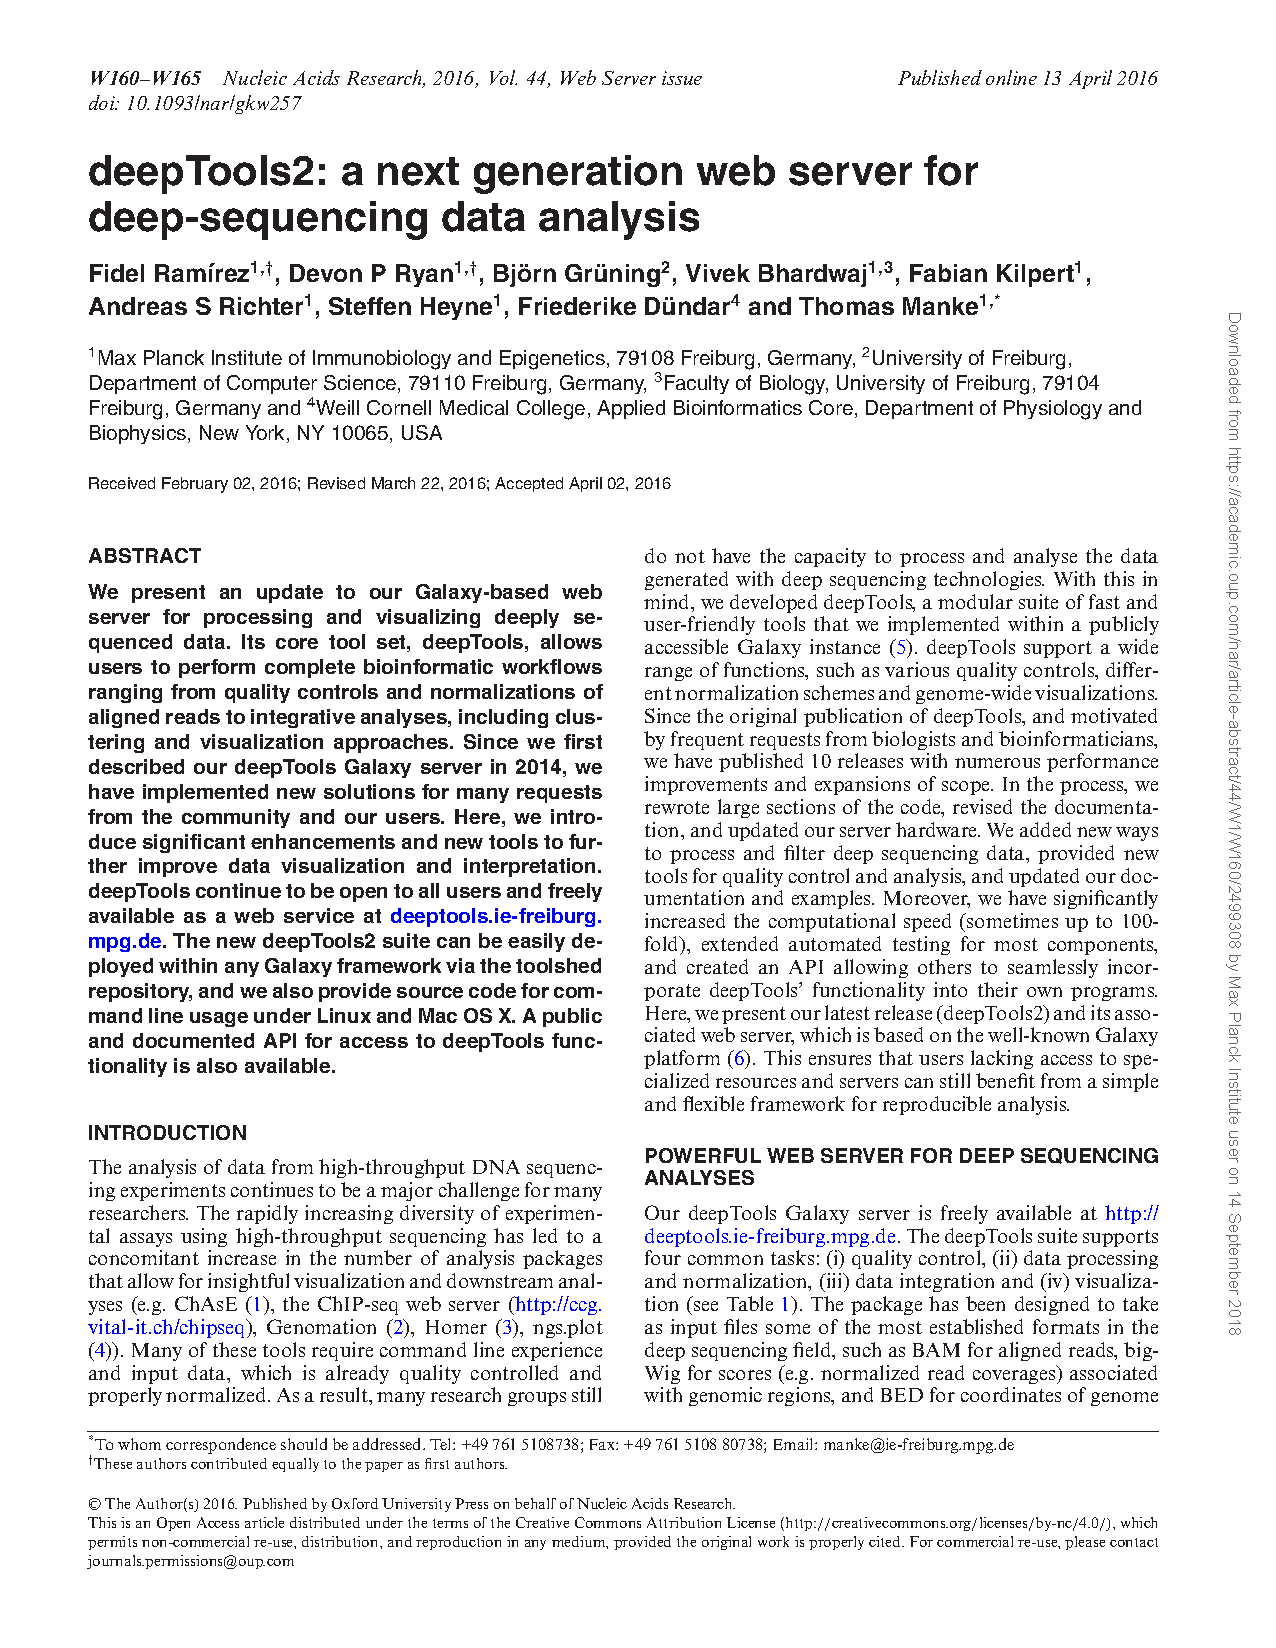
\includepdf[scale=0.9,pages=-,pagecommand={}, offset=0.3cm 0cm]{manuscripts/NAR_2016_article.pdf}

\section{snakePipes enables reproducible epigenomic
analysis}\label{snakepipes-enables-reproducible-epigenomic-analysis}

I developed the allele-specific and HiC workflows and contributed to
DNA-mapping, ChIP-seq, ATAC-seq and RNA-seq workflows and documentation.
I performed the analysis, prepared the figures and wrote the manuscript
with input from all authors.


\includepdf[scale=0.9,pages=-,pagecommand={}, offset=0.3cm 0cm]{manuscripts/snakepipes_manuscript_10-09-2018.pdf}

\chapter{Supplemental information}\label{supplemental-information}

\chapter{Academic Vita}\label{academic-vita}

\backmatter

\chapter*{References}\label{references}
\addcontentsline{toc}{chapter}{References}

\markboth{References}{References}

\noindent

\setlength{\parindent}{-0.20in} \setlength{\leftskip}{0.20in}
\setlength{\parskip}{8pt}

\hypertarget{refs}{}
\hypertarget{ref-angel2000}{}
Angel, E. (2000). \emph{Interactive computer graphics : A top-down
approach with opengl}. Boston, MA: Addison Wesley Longman.

\hypertarget{ref-angel2001}{}
Angel, E. (2001a). \emph{Batch-file computer graphics : A bottom-up
approach with quicktime}. Boston, MA: Wesley Addison Longman.

\hypertarget{ref-angel2002a}{}
Angel, E. (2001b). \emph{Test second book by angel}. Boston, MA: Wesley
Addison Longman.


% Index?

\end{document}
